我们住在大楼里,冬天有人开暖气、空调、地暖等取暖,夏天有人开空调制冷清凉。
本文根据传热学知识,考虑以下方面分析邻居们制冷、制热对所处房间温度的影响,并利用代码和可视化方法分析房间温度的变化情况。

\subsection{初始条件以及边界条件}
初始条件:初始房间温度与环境温度相同,冬天为10摄氏度,夏天为35摄氏度。

边界条件:在分析隔壁房间温度时考虑墙体的隔热效果,在分析所处房间的温度时考虑墙壁的导热效果。

\subsection{房间简化模型}
本文为了计算方便,将房间简化为$3m\times3m\times3m$的正方体,同时设定房间墙壁厚度为$0.2m$,具体布局如下图所示:

\begin{figure}[h]
    \centering
    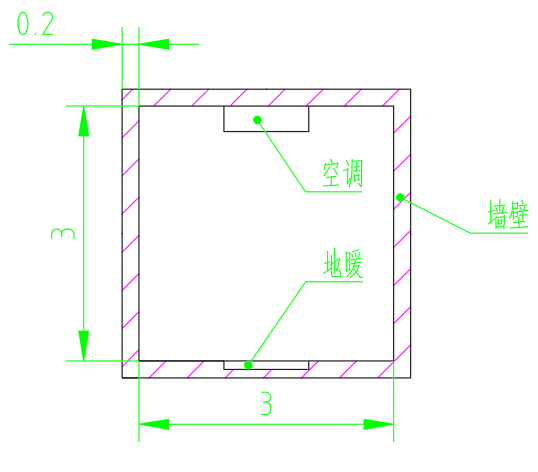
\includegraphics[scale = 0.5]{figures/房间模型.png}
    \caption{房间布局简化模型}
    \label{fig:Room}
\end{figure}

其中空调设置为扫风模式,简化为一个恒温热源以匀速在空间内上下移动,形成第一类边界条件,热源温度即为空调设定温度。

地暖简化为热流大小固定的热源,忽略其厚度,与墙壁一起组成第二类边界条件。

\subsection{传热过程}
因为同时考虑四面墙壁的导热过程以及空调和地暖的工作,其中空调设置为随时间变化的扫风模式,该传热问题为二维非稳态传热过程,使用有限差分法进行求解。


